%=========================================================
% MODULE 1 : MODERN COMPUTING APPROACHES
% Part 1 : Evolution of Computing
% Text Book 1: Sections 1.1, 1.1.1, 1.1.2
% Kai Hwang, Geoffrey C. Fox and Jack J. Dongarra,
% Distributed and Cloud Computing, Morgan Kaufmann, 2012
%=========================================================

%=========================================================
\section{Module 1: Scalable Computing over the Internet}
%=========================================================

\begin{frame}{Module 1 - Evolution of Computing: What We Will Learn}
\begin{enumerate}
\item<1-> \textbf{Scalable Computing over the Internet} --- why one computer is no longer enough.
\item<2-> \textbf{The Age of Internet Computing:}
    \begin{itemize}
    \item Platform evolution (five generations of computers)
    \item High-Performance Computing (HPC) and High-Throughput Computing (HTC)
    \item Three new computing paradigms and computing paradigm distinctions
    \item Distributed system families and their design objectives
    \end{itemize}
\item<3-> \textbf{Scalable Computing Trends and New Paradigms:}
    \begin{itemize}
    \item Degrees of parallelism, innovative applications
    \item The trend toward utility computing and the hype cycle of new technologies
    \end{itemize}
\end{enumerate}
\end{frame}

%---------------------------------------------------------
\begin{frame}{Scalable Computing over the Internet}
\begin{block}{Key Idea}
Instead of using one \textbf{centralized} computer, a \textbf{parallel and distributed} computing system uses \textbf{many computers} working together over the Internet to solve large-scale problems.
\end{block}
\vspace{0.2cm}
\begin{enumerate}
\item<1-> Over the past 60 years, computing has changed in its \textbf{machine architecture}, \textbf{operating system platform}, \textbf{network connectivity}, and \textbf{application workload}.
\item<2-> As a result, computing has become \textbf{data-intensive} and \textbf{network-centric}.
\item<3-> Large-scale Internet applications (search, e-mail, online banking, social media) have greatly improved the \textbf{quality of life} and information services in society.
\item<4-> \textbf{Everyday example:} A single Google search is answered by thousands of servers working together, not by one computer.
\end{enumerate}
\end{frame}

%=========================================================
\subsection{The Age of Internet Computing}
%=========================================================

\begin{frame}{The Age of Internet Computing}
\begin{enumerate}
\item<1-> \textbf{Billions of people} use the Internet every day.
\item<2-> Supercomputer sites and large \textbf{data centers} must serve huge numbers of users \textbf{at the same time} (concurrently).
\item<3-> The \textbf{Linpack Benchmark}, traditionally used to rank HPC systems by raw speed, is \textbf{no longer the best measure} for such workloads.
\item<4-> Cloud computing instead demands \textbf{High-Throughput Computing (HTC)} systems built with parallel and distributed technologies.
\item<5-> Data centers must be upgraded with:
    \begin{itemize}
    \item Fast servers
    \item Large storage systems
    \item High-bandwidth networks
    \end{itemize}
\end{enumerate}
\end{frame}

%---------------------------------------------------------
\begin{frame}{The Platform Evolution: Five Generations}
\begin{enumerate}
\item<1-> Computer technology has gone through \textbf{five generations}; each lasted \textbf{10--20 years}, and successive generations \textbf{overlapped by about 10 years}.
\end{enumerate}
\begin{table}
\centering
\renewcommand{\arraystretch}{1.25}
\scriptsize
\begin{tabular}{|p{2cm}|p{3.6cm}|p{4.2cm}|p{3.4cm}|}
\hline
\textbf{Period} & \textbf{Platform} & \textbf{Examples} & \textbf{Main Users} \\ \hline
1950--1970 & Mainframes & IBM 360, CDC 6400 & Large businesses, government \\ \hline
1960--1980 & Minicomputers (lower cost) & DEC PDP 11, VAX Series & Small businesses, colleges \\ \hline
1970--1990 & Personal computers & PCs built with VLSI microprocessors & Individuals, offices \\ \hline
1980--2000 & Portable \& pervasive devices & Laptops, wired and wireless devices & Mobile users \\ \hline
Since 1990 & HPC and HTC systems & Clusters, grids, Internet clouds & Consumers and web-scale services \\ \hline
\end{tabular}
\end{table}
\begin{enumerate}\setcounter{enumi}{1}
\item<2-> \textbf{General trend:} Leverage \textbf{shared web resources} and \textbf{massive amounts of data} over the Internet.
\end{enumerate}
\end{frame}

%---------------------------------------------------------
\begin{frame}{Evolutionary Trend toward Parallel, Distributed, and Cloud Computing}
\begin{columns}[T]
\begin{column}{0.50\textwidth}
\begin{figure}
\centering
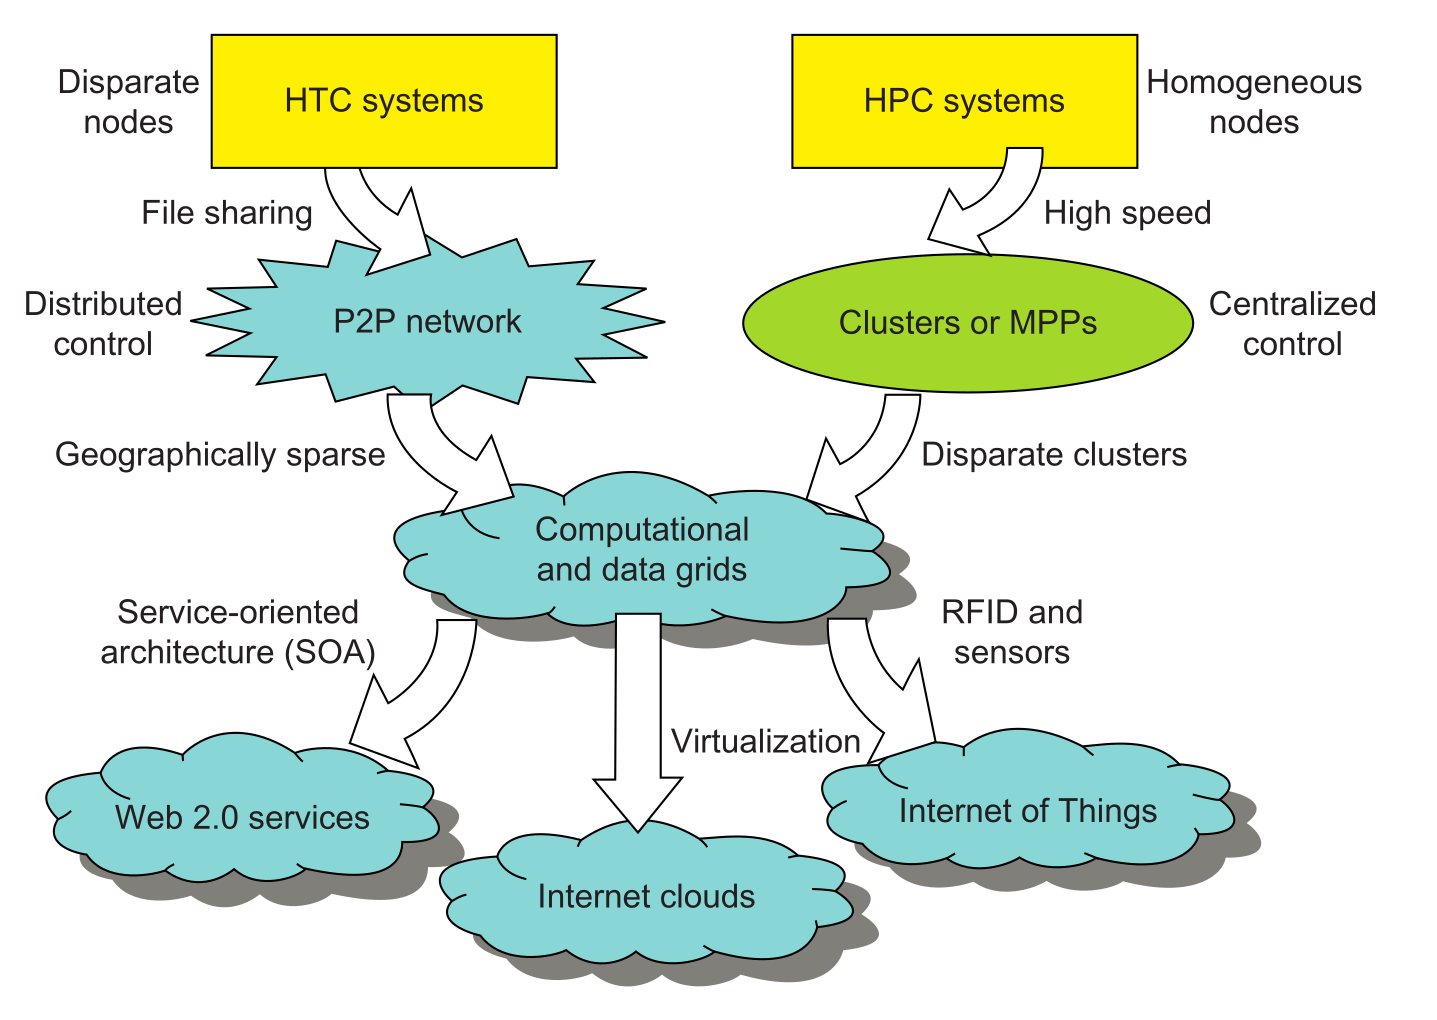
\includegraphics[width=0.92\linewidth]{images/Fig1_1_evolution_trend.png}
\caption{\scriptsize Evolutionary trend toward parallel, distributed, and cloud computing (Fig.\ 1.1)}
\end{figure}
\end{column}
\begin{column}{0.48\textwidth}
\begin{enumerate}\small
\item<1-> The figure has \textbf{two starting points}: \textbf{HPC systems} (right) and \textbf{HTC systems} (left).
\item<2-> \textbf{HPC side:} Supercomputers (\textbf{MPPs}) are gradually replaced by \textbf{clusters} of cooperative computers to \textbf{share resources}.
\item<3-> \textbf{HTC side:} \textbf{Peer-to-peer (P2P)} networks are formed for distributed file sharing and content delivery.
\item<4-> Clustering and P2P technologies together lead to \textbf{computational and data grids}.
\item<5-> Grids in turn lead to \textbf{Web 2.0 services}, \textbf{Internet clouds}, and the \textbf{Internet of Things}.
\end{enumerate}
\end{column}
\end{columns}
\end{frame}

%---------------------------------------------------------
\begin{frame}{Reading Figure 1.1: Labels on the Arrows}
\begin{table}
\centering
\renewcommand{\arraystretch}{1.3}
\scriptsize
\begin{tabular}{|p{3.2cm}|p{4.6cm}|p{4.6cm}|}
\hline
\textbf{Feature} & \textbf{HPC Path (Clusters / MPPs)} & \textbf{HTC Path (P2P Networks)} \\ \hline
Type of nodes & \textbf{Homogeneous} (same kind of computers) & \textbf{Disparate} (different kinds of computers) \\ \hline
Control & \textbf{Centralized} control & \textbf{Distributed} control \\ \hline
Location & Physically close (one room / building) & \textbf{Geographically sparse} (spread worldwide) \\ \hline
Purpose & \textbf{High speed} & \textbf{File sharing} \\ \hline
\end{tabular}
\end{table}
\begin{enumerate}
\item<1-> \textbf{Disparate clusters} and \textbf{geographically sparse} P2P networks merge into \textbf{grids}.
\item<2-> From grids: \textbf{SOA} $\rightarrow$ Web 2.0 services; \textbf{Virtualization} $\rightarrow$ Internet clouds; \textbf{RFID and sensors} $\rightarrow$ Internet of Things.
\item<3-> A \textbf{cluster} is a collection of homogeneous compute nodes physically connected close to one another (detailed later in this module).
\end{enumerate}
\end{frame}

%---------------------------------------------------------
\begin{frame}{High-Performance Computing (HPC)}
\begin{block}{HPC}
Computing systems that emphasize \textbf{raw speed} performance --- how fast a single large problem can be solved.
\end{block}
\vspace{0.2cm}
\begin{enumerate}
\item<1-> HPC speed has grown from \textbf{Gflops} (early 1990s) to \textbf{Pflops} (2010).
    \begin{itemize}
    \item flops = floating-point operations per second; Giga = $10^9$, Peta = $10^{15}$.
    \end{itemize}
\item<2-> Growth was driven by \textbf{scientific, engineering, and manufacturing} communities.
\item<3-> The \textbf{Top 500} list ranks the world's most powerful computers by floating-point speed in the \textbf{Linpack benchmark}.
\item<4-> However, supercomputer users are \textbf{less than 10\%} of all computer users.
\item<5-> \textbf{Example:} Weather forecasting, earthquake simulation, genome analysis.
\end{enumerate}
\end{frame}

%---------------------------------------------------------
\begin{frame}{High-Throughput Computing (HTC)}
\begin{block}{HTC}
Computing systems that emphasize \textbf{high-flux computing} --- the \textbf{number of tasks completed per unit of time}.
\end{block}
\vspace{0.2cm}
\begin{enumerate}
\item<1-> Market-oriented high-end computing is shifting from an \textbf{HPC paradigm} to an \textbf{HTC paradigm}.
\item<2-> Main applications: \textbf{Internet searches} and \textbf{web services} used by millions of users simultaneously.
\item<3-> HTC must improve batch processing speed \textbf{and} address:
    \begin{itemize}
    \item Cost
    \item Energy savings
    \item Security
    \item Reliability
    \end{itemize}
\item<4-> \textbf{Example:} Millions of students checking exam results on a university website at the same time.
\end{enumerate}
\end{frame}

%---------------------------------------------------------
\begin{frame}{HPC versus HTC: A Comparison}
\begin{table}
\centering
\renewcommand{\arraystretch}{1.35}
\scriptsize
\begin{tabular}{|p{3cm}|p{5cm}|p{5cm}|}
\hline
\textbf{Aspect} & \textbf{High-Performance Computing} & \textbf{High-Throughput Computing} \\ \hline
Goal & Solve \textbf{one big problem fast} & Complete \textbf{many tasks} per unit time \\ \hline
Measure & Speed (flops, Linpack benchmark) & Throughput (tasks completed per unit time) \\ \hline
Typical systems & Supercomputers, MPPs, clusters & P2P networks, clouds, web service platforms \\ \hline
Typical users & Scientists and engineers ($<$10\% of users) & General Internet users (millions) \\ \hline
Applications & Simulations, weather forecasting & Web search, e-commerce, social networks \\ \hline
\end{tabular}
\end{table}
\begin{enumerate}
\item<1-> \textbf{Analogy:} HPC is a \textbf{racing car} (one passenger, very fast); HTC is a \textbf{metro train} (thousands of passengers per hour).
\end{enumerate}
\end{frame}

%---------------------------------------------------------
\begin{frame}{Three New Computing Paradigms}
\begin{enumerate}
\item<1-> \textbf{Service-Oriented Architecture (SOA) $\rightarrow$ Web 2.0 services:}
    \begin{itemize}
    \item Software is offered as \textbf{services} over the web (e.g., online maps, payment services).
    \end{itemize}
\item<2-> \textbf{Virtualization $\rightarrow$ Internet clouds:}
    \begin{itemize}
    \item Advances in virtualization made it possible to grow \textbf{Internet clouds} as a new paradigm.
    \end{itemize}
\item<3-> \textbf{RFID, GPS, and sensor technologies $\rightarrow$ Internet of Things (IoT):}
    \begin{itemize}
    \item Maturity of radio-frequency identification (RFID), Global Positioning System (GPS), and sensors triggered the development of the IoT.
    \end{itemize}
\item<4-> The differences among clusters, grids, P2P systems, and clouds \textbf{may blur} in the future.
\end{enumerate}
\end{frame}

%---------------------------------------------------------
\begin{frame}{How the Idea of a ``Computer'' Has Changed}
\begin{table}
\centering
\renewcommand{\arraystretch}{1.4}
\scriptsize
\begin{tabular}{|p{1.2cm}|p{4.3cm}|p{7cm}|}
\hline
\textbf{Year} & \textbf{Person} & \textbf{Idea} \\ \hline
1969 & Leonard Kleinrock (UCLA) & Computer networks would grow into \textbf{computer utilities}, serving homes and offices like electricity and telephone. \\ \hline
1984 & John Gage (Sun Microsystems) & ``The network is the computer.'' \\ \hline
2008 & David Patterson (UC Berkeley) & ``The data center is the computer.'' \\ \hline
Recent & Rajkumar Buyya (Univ.\ of Melbourne) & ``The cloud is the computer.'' \\ \hline
\end{tabular}
\end{table}
\begin{enumerate}
\item<1-> The ``computer'' has moved from a \textbf{single machine} $\rightarrow$ a \textbf{network} $\rightarrow$ a \textbf{data center} $\rightarrow$ the \textbf{cloud}.
\item<2-> Building software used as a \textbf{service by millions} is very different from distributing software to run on individual PCs.
\end{enumerate}
\end{frame}

%---------------------------------------------------------
\begin{frame}{Computing Paradigm Distinctions (1/2)}
\begin{enumerate}
\item<1-> \textbf{Centralized computing:}
    \begin{itemize}
    \item All resources (processors, memory, storage) are in \textbf{one physical system}.
    \item Resources are fully shared and \textbf{tightly coupled} within one integrated OS.
    \item Many data centers and supercomputers are centralized systems.
    \end{itemize}
\item<2-> \textbf{Parallel computing:}
    \begin{itemize}
    \item Processors are either \textbf{tightly coupled} (centralized shared memory) or \textbf{loosely coupled} (distributed memory).
    \item Processors communicate through \textbf{shared memory} or \textbf{message passing}.
    \item The computer is called a \textbf{parallel computer}; its programs are \textbf{parallel programs}; writing them is \textbf{parallel programming}.
    \end{itemize}
\end{enumerate}
\end{frame}

%---------------------------------------------------------
\begin{frame}{Computing Paradigm Distinctions (2/2)}
\begin{enumerate}
\item<1-> \textbf{Distributed computing:}
    \begin{itemize}
    \item A distributed system has \textbf{multiple autonomous computers}, each with its \textbf{own private memory}, connected by a network.
    \item Information is exchanged through \textbf{message passing}.
    \item Programs are \textbf{distributed programs}; writing them is \textbf{distributed programming}.
    \end{itemize}
\item<2-> \textbf{Cloud computing:}
    \begin{itemize}
    \item An Internet cloud can be either \textbf{centralized} or \textbf{distributed}.
    \item It applies parallel or distributed computing, or both.
    \item Built with \textbf{physical or virtualized} resources over large data centers.
    \item Some consider it a form of \textbf{utility computing} or \textbf{service computing}.
    \end{itemize}
\end{enumerate}
\end{frame}

%---------------------------------------------------------
\begin{frame}{Computing Paradigms at a Glance}
\begin{table}
\centering
\renewcommand{\arraystretch}{1.35}
\scriptsize
\begin{tabular}{|p{2.4cm}|p{3.2cm}|p{3.4cm}|p{3.8cm}|}
\hline
\textbf{Paradigm} & \textbf{Memory} & \textbf{Communication} & \textbf{Everyday Analogy} \\ \hline
Centralized & One system, fully shared & Within one OS & One chef cooking in one kitchen \\ \hline
Parallel & Shared or distributed & Shared memory / message passing & Many chefs in one kitchen cooking one meal \\ \hline
Distributed & Private memory per computer & Message passing over a network & Branches of a restaurant chain coordinating by phone \\ \hline
Cloud & Centralized or distributed & Over the Internet & Ordering food online; you never see the kitchen \\ \hline
\end{tabular}
\end{table}
\begin{enumerate}
\item<1-> \textbf{Distributed computing} is the \textbf{opposite} of centralized computing.
\item<2-> Parallel computing \textbf{overlaps} with distributed computing; cloud computing overlaps with all three.
\end{enumerate}
\end{frame}

%---------------------------------------------------------
\begin{frame}{Related Terms}
\begin{enumerate}
\item<1-> \textbf{Concurrent computing / programming:} Usually refers to the \textbf{union} of parallel and distributed computing.
\item<2-> \textbf{Ubiquitous computing:} Computing with pervasive devices at \textbf{any place and any time}, using wired or wireless communication.
\item<3-> \textbf{Internet of Things (IoT):} A networked connection of \textbf{everyday objects} --- computers, sensors, humans, etc. --- supported by Internet clouds.
\item<4-> \textbf{Internet computing:} The broadest term, covering \textbf{all computing paradigms} over the Internet.
\item<5-> \textbf{Example of IoT:} A smart watch sending your step count to a phone app, which stores it in the cloud.
\end{enumerate}
\end{frame}

%---------------------------------------------------------
\begin{frame}{Distributed System Families}
\begin{enumerate}
\item<1-> Since the mid-1990s, P2P networks and networks of clusters were consolidated into national projects called \textbf{computational grids} or \textbf{data grids}.
\item<2-> \textbf{Internet clouds} result from moving desktop computing to \textbf{service-oriented computing} using server clusters and huge databases at data centers.
\item<3-> Grids and clouds place great emphasis on \textbf{resource sharing} in hardware, software, and data sets.
\item<4-> \textbf{Scale of these systems:}
    \begin{itemize}
    \item \textbf{Tianhe-1A} cluster (China, Oct.\ 2010): 86,016 CPU cores and 3,211,264 GPU cores.
    \item The largest computational grid connects up to \textbf{hundreds of server clusters}.
    \item A typical P2P network may involve \textbf{millions of client machines}.
    \item Experimental cloud clusters have been built with \textbf{thousands of processing nodes}.
    \end{itemize}
\end{enumerate}
\end{frame}

%---------------------------------------------------------
\begin{frame}{Design Objectives for Future HPC and HTC Systems}
\begin{enumerate}
\item<1-> Future systems will need \textbf{multicore / many-core} processors handling many threads per core.
\item<2-> System efficiency depends on \textbf{speed}, \textbf{programming}, and \textbf{energy} (throughput per watt).
\end{enumerate}
\begin{table}
\centering
\renewcommand{\arraystretch}{1.3}
\scriptsize
\begin{tabular}{|p{3.2cm}|p{10cm}|}
\hline
\textbf{Objective} & \textbf{What It Measures} \\ \hline
Efficiency & Utilization of resources; for HPC via massive parallelism, for HTC via job throughput, data access, storage, and power efficiency. \\ \hline
Dependability & Reliability and self-management from chip to application level; service with \textbf{QoS} assurance even under failures. \\ \hline
Adaptation in the programming model & Ability to support \textbf{billions of job requests} over massive data sets and virtualized cloud resources. \\ \hline
Flexibility in application deployment & Ability to run well in both \textbf{HPC} (science and engineering) and \textbf{HTC} (business) applications. \\ \hline
\end{tabular}
\end{table}
\end{frame}

%=========================================================
\subsection{Scalable Computing Trends and New Paradigms}
%=========================================================

\begin{frame}{Scalable Computing Trends}
\begin{enumerate}
\item<1-> Designers try to \textbf{predict} the capabilities of future systems from technology trends (e.g., Jim Gray's paper \textit{Rules of Thumb in Data Engineering}).
\item<2-> \textbf{Moore's law:} Processor speed \textbf{doubles every 18 months}.
    \begin{itemize}
    \item Valid for the last 30 years; whether it continues is uncertain.
    \end{itemize}
\item<3-> \textbf{Gilder's law:} Network bandwidth has \textbf{doubled each year}.
\item<4-> The excellent \textbf{price/performance ratio} of commodity hardware (desktops, notebooks, tablets) has driven the use of commodity technologies in \textbf{large-scale computing}.
\item<5-> Distributed systems emphasize both \textbf{resource distribution} and \textbf{concurrency}, i.e., a high \textbf{degree of parallelism (DoP)}.
\end{enumerate}
\end{frame}

%---------------------------------------------------------
\begin{frame}{Degrees of Parallelism}
\begin{table}
\centering
\renewcommand{\arraystretch}{1.3}
\scriptsize
\begin{tabular}{|p{3.8cm}|p{9.4cm}|}
\hline
\textbf{Level} & \textbf{Description} \\ \hline
Bit-Level Parallelism (BLP) & Converts bit-serial processing to word-level; 4-bit $\rightarrow$ 8, 16, 32, 64-bit CPUs. \\ \hline
Instruction-Level Parallelism (ILP) & Processor executes \textbf{multiple instructions at once}; via pipelining, superscalar, VLIW, multithreading. \\ \hline
Data-Level Parallelism (DLP) & One instruction on \textbf{many data items}; via SIMD and vector machines. \\ \hline
Task-Level Parallelism (TLP) & Different \textbf{tasks} on different cores of multicore processors (CMPs). \\ \hline
Job-Level Parallelism (JLP) & Whole \textbf{jobs} on different computers in distributed processing. \\ \hline
\end{tabular}
\end{table}
\begin{enumerate}
\item<1-> BLP, ILP, and DLP are well supported by hardware and compilers.
\item<2-> TLP is \textbf{less successful} because programming multicore processors efficiently is difficult.
\item<3-> \textbf{Coarse-grain} parallelism (JLP) is built on top of \textbf{fine-grain} parallelism (BLP, ILP).
\end{enumerate}
\end{frame}

%---------------------------------------------------------
\begin{frame}{Degrees of Parallelism: An Everyday View}
\begin{enumerate}
\item<1-> \textbf{BLP:} Adding two numbers 64 bits at a time instead of one bit at a time.
\item<2-> \textbf{ILP:} An assembly line --- one instruction is fetched while another is being executed.
\item<3-> \textbf{DLP:} Increasing the brightness of \textbf{every pixel} of a photo with one instruction.
\item<4-> \textbf{TLP:} Your phone plays music on one core while downloading a file on another.
\item<5-> \textbf{JLP:} A cloud runs thousands of users' jobs on thousands of separate servers.
\item<6-> Granularity \textbf{increases} as we move from parallel processing (inside one computer) to distributed processing (across many computers).
\end{enumerate}
\end{frame}

%---------------------------------------------------------
\begin{frame}{Innovative Applications}
\begin{table}
\centering
\renewcommand{\arraystretch}{1.25}
\scriptsize
\begin{tabular}{|p{3.6cm}|p{9.6cm}|}
\hline
\textbf{Domain} & \textbf{Specific Applications} \\ \hline
Science and engineering & Scientific simulations, genomic analysis; earthquake prediction, global warming, weather forecasting \\ \hline
Business, education, services industry, and health care & Telecommunication, content delivery, e-commerce; banking, stock exchanges, transaction processing; air traffic control, electric power grids, distance education; health care, hospital automation, telemedicine \\ \hline
Internet and web services, and government & Internet search, data centers, decision-making systems; traffic monitoring, worm containment, cyber security; digital government, online tax return processing, social networking \\ \hline
Mission-critical applications & Military command and control, intelligent systems, crisis management \\ \hline
\end{tabular}
\caption{\scriptsize Applications of high-performance and high-throughput systems (Table 1.1)}
\end{table}
\end{frame}

%---------------------------------------------------------
\begin{frame}{Requirements of Innovative Applications}
\begin{enumerate}
\item<1-> HPC and HTC systems need \textbf{transparency}: the user should not have to worry about:
    \begin{itemize}
    \item Data access and resource allocation
    \item Process location and concurrency in execution
    \item Job replication and failure recovery
    \end{itemize}
\item<2-> Almost all applications demand \textbf{computing economics}, \textbf{web-scale data collection}, \textbf{system reliability}, and \textbf{scalable performance}.
\item<3-> \textbf{Banking example:}
    \begin{itemize}
    \item Distributed transaction processing is common in banking and finance.
    \item Transactions form about \textbf{90\%} of the market for reliable banking systems.
    \item Keeping \textbf{replicated transaction records consistent} is crucial in real-time banking.
    \end{itemize}
\item<4-> Challenges: lack of software support, \textbf{network saturation}, and \textbf{security threats}.
\end{enumerate}
\end{frame}

%---------------------------------------------------------
\begin{frame}{The Trend toward Utility Computing}
\begin{columns}[T]
\begin{column}{0.52\textwidth}
\begin{figure}
\centering
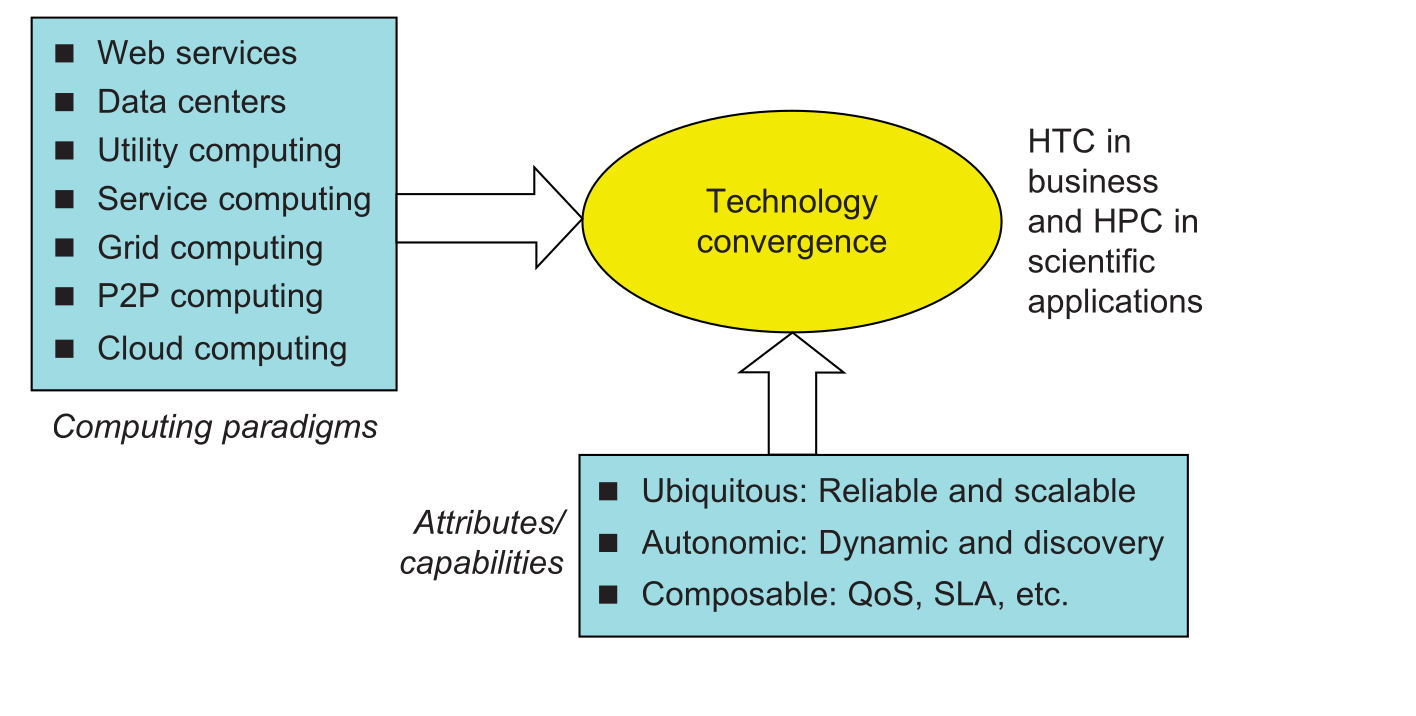
\includegraphics[width=\linewidth]{images/Fig1_2_computer_utilities.png}
\caption{\scriptsize The vision of computer utilities in modern distributed computing systems (Fig.\ 1.2)}
\end{figure}
\end{column}
\begin{column}{0.46\textwidth}
\begin{enumerate}\small
\item<1-> \textbf{Left box:} Computing paradigms --- web services, data centers, utility, service, grid, P2P, and cloud computing.
\item<2-> \textbf{Bottom box:} Common attributes --- \textbf{ubiquitous}, \textbf{autonomic}, and \textbf{composable}.
\item<3-> Both feed into \textbf{technology convergence}.
\item<4-> The result: \textbf{HTC in business} and \textbf{HPC in scientific} applications.
\end{enumerate}
\end{column}
\end{columns}
\end{frame}

%---------------------------------------------------------
\begin{frame}{Common Characteristics of These Paradigms}
\begin{enumerate}
\item<1-> \textbf{Ubiquitous:} Present everywhere in daily life; \textbf{reliability} and \textbf{scalability} are the two major design objectives.
\item<2-> \textbf{Autonomic:} Can \textbf{self-organize} to support \textbf{dynamic discovery} of resources.
\item<3-> \textbf{Composable:} Can be combined with guaranteed \textbf{QoS} (Quality of Service) and \textbf{SLAs} (Service-Level Agreements).
\item<4-> Together, these paradigms and attributes realize the \textbf{computer utility vision}.
\end{enumerate}
\end{frame}

%---------------------------------------------------------
\begin{frame}{Utility Computing}
\begin{block}{Utility Computing}
A business model in which customers receive computing resources from a \textbf{paid service provider}, just like electricity or water.
\end{block}
\vspace{0.2cm}
\begin{enumerate}
\item<1-> All grid and cloud platforms are regarded as \textbf{utility service providers}.
\item<2-> Cloud computing is a \textbf{broader concept} than utility computing.
\item<3-> Distributed cloud applications run on any available servers in some edge networks.
\item<4-> \textbf{Technological challenges} include network-efficient processors, scalable memory and storage, distributed OSes, virtualization middleware, new programming models, and effective resource management.
\item<5-> \textbf{Analogy:} You pay the electricity bill for units consumed; you do not build a power plant at home.
\end{enumerate}
\end{frame}

%---------------------------------------------------------
\begin{frame}{The Hype Cycle of New Technologies}
\begin{figure}
\centering
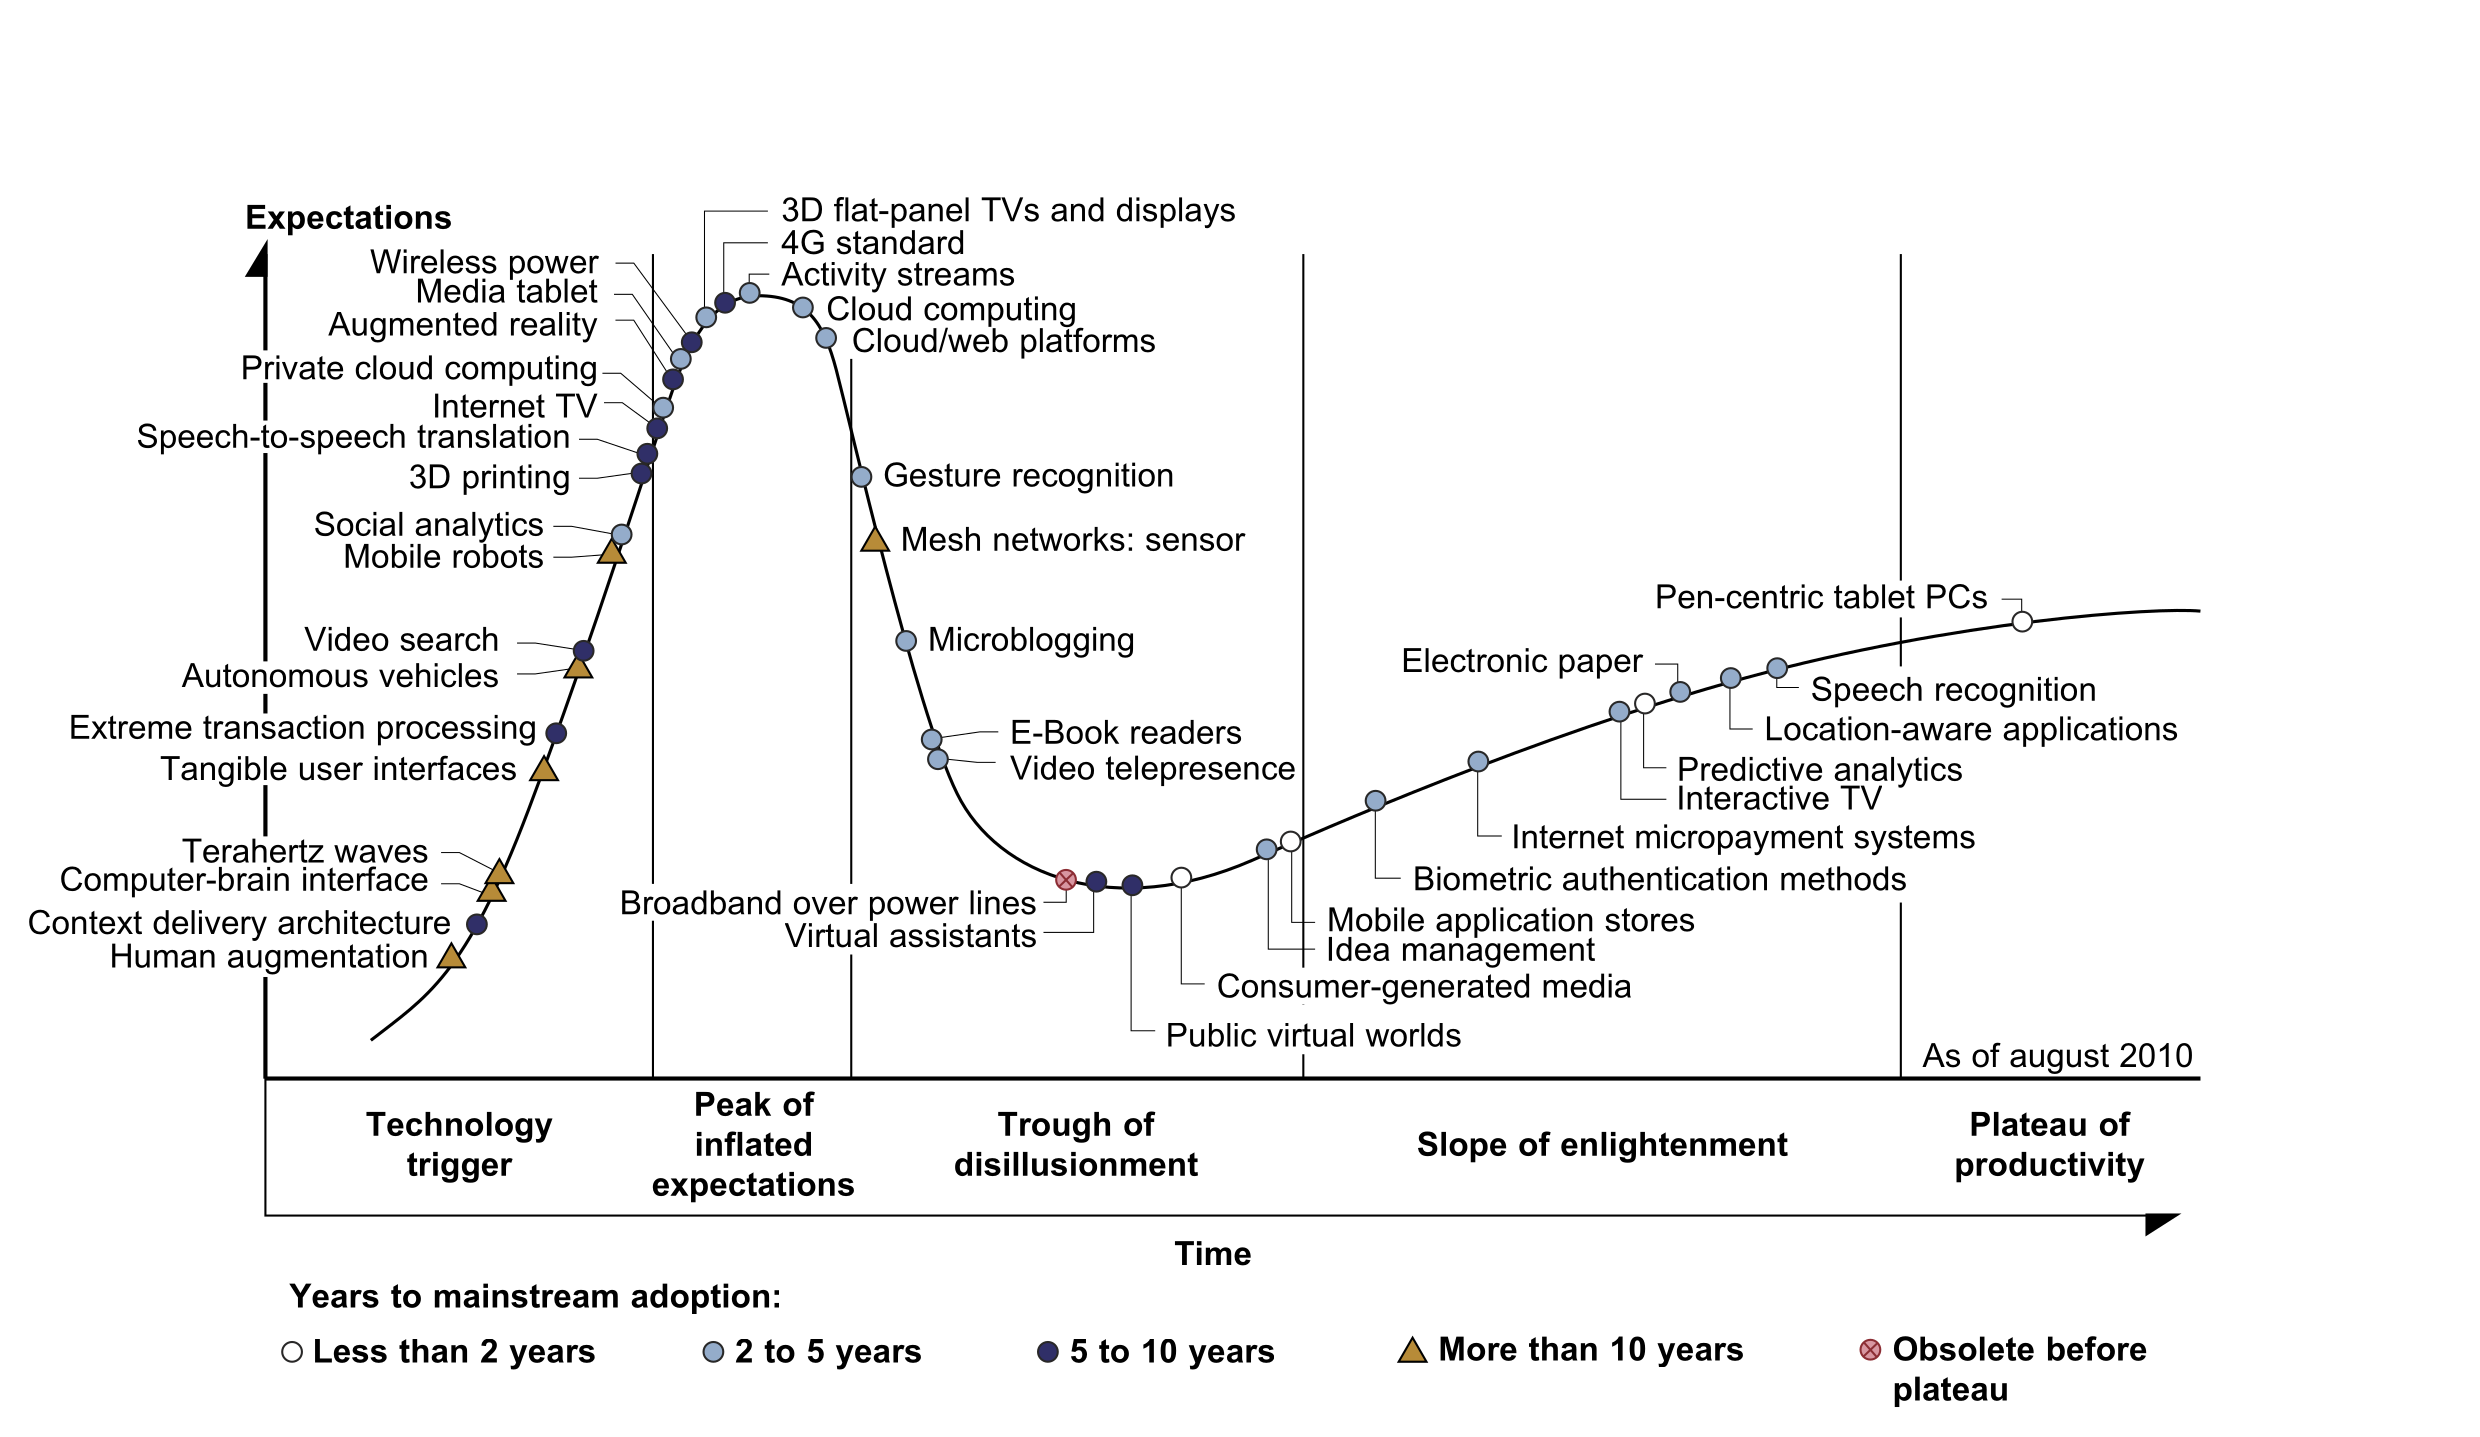
\includegraphics[height=0.70\textheight]{images/Fig1_3_hype_cycle.png}
\caption{\scriptsize Hype cycle for emerging technologies, 2010 (Fig.\ 1.3; source: Gartner, Inc., 2010, as reproduced in Text Book 1)}
\end{figure}
\end{frame}

%---------------------------------------------------------
\begin{frame}{Five Stages of the Hype Cycle}
\begin{enumerate}
\item<1-> \textbf{Technology trigger:} A new technology appears; expectations begin to rise.
\item<2-> \textbf{Peak of inflated expectations:} Expectations rise sharply --- often beyond reality.
\item<3-> \textbf{Trough of disillusionment:} After a short period, expectations drop into a valley.
\item<4-> \textbf{Slope of enlightenment:} Expectations increase steadily over a long period as real uses are understood.
\item<5-> \textbf{Plateau of productivity:} The technology reaches \textbf{mainstream adoption}.
\item<6-> Once a technology climbs the slope of enlightenment, it may reach the plateau within \textbf{two to five years}.
\end{enumerate}
\end{frame}

%---------------------------------------------------------
\begin{frame}{Reading the Hype Cycle: Symbols and Examples (2010)}
\begin{table}
\centering
\renewcommand{\arraystretch}{1.25}
\scriptsize
\begin{tabular}{|p{3.2cm}|p{3.4cm}|p{6.4cm}|}
\hline
\textbf{Symbol} & \textbf{Years to Mainstream} & \textbf{Example (as of August 2010)} \\ \hline
Hollow circle & Less than 2 years & Consumer-generated media (in the trough) \\ \hline
Gray circle & 2 to 5 years & Internet micropayment systems; cloud computing \\ \hline
Solid (dark) circle & 5 to 10 years & 3D printing (rising expectations) \\ \hline
Triangle & More than 10 years & Mesh network sensors \\ \hline
Crossed circle & Obsolete before plateau & Broadband over power lines \\ \hline
\end{tabular}
\end{table}
\begin{enumerate}
\item<1-> In 2010, \textbf{cloud technology} had just crossed the \textbf{peak} and was expected to reach productivity in \textbf{2--5 years}.
\item<2-> Other promising technologies then: biometric authentication, interactive TV, speech recognition, predictive analytics, media tablets.
\item<3-> \textbf{Think:} Where would you place cloud computing, AI chatbots, or 3D printing on the hype cycle \textbf{today}?
\end{enumerate}
\end{frame}

%=========================================================
\subsection{Summary}
%=========================================================

\begin{frame}{Summary}
\begin{enumerate}
\item<1-> Computing has evolved from \textbf{mainframes} to \textbf{clusters, grids, and Internet clouds} over five generations.
\item<2-> \textbf{HPC} focuses on raw speed; \textbf{HTC} focuses on the number of tasks completed per unit time.
\item<3-> \textbf{SOA, virtualization, and RFID/GPS/sensors} gave rise to Web 2.0 services, clouds, and the IoT.
\item<4-> Centralized, parallel, distributed, and cloud computing differ in \textbf{how resources and memory are shared}.
\item<5-> Parallelism has grown from \textbf{bit-level} to \textbf{job-level}.
\item<6-> Modern paradigms are \textbf{ubiquitous, autonomic, and composable}, realizing the \textbf{computer utility} vision.
\item<7-> New technologies follow a \textbf{hype cycle} before reaching mainstream adoption.
\end{enumerate}
\end{frame}

%---------------------------------------------------------
\begin{frame}{Review Questions}
\begin{enumerate}\small
\item List the five generations of computer platforms with one example each.
\item Differentiate between HPC and HTC systems with suitable examples.
\item Explain the evolutionary trend shown in Figure 1.1.
\item Distinguish centralized, parallel, distributed, and cloud computing.
\item What are the three new computing paradigms? What enabled each of them?
\item Explain the five degrees of parallelism.
\item Explain the vision of computer utilities with a neat diagram (Figure 1.2).
\item Describe the five stages of the hype cycle of new technologies.
\end{enumerate}
\end{frame}
